\documentclass{report}
\usepackage[utf8]{inputenc}

\title{NSF Report 2020 Addendum}
\author{Alexander Salois, Dr Ioannis Roudas (PI)}
\date{September 2020}

\usepackage{natbib}
\usepackage{graphicx}
\usepackage{booktabs}

\begin{document}
 
\maketitle

\section{Overview of Tasks at MSU}
Task 1: Development of a physical-layer-aware network simulation tool for pace Division Multiplexing (SDM) Wavelength Divsion Multiplexing (WDM) optical networks
In this task, we will perform computer-aided design based on the worst optical path in the network assuming long-haul coherent optical communication systems.  An example model that was used to simulate long haul communications can be seen below in figure \ref{fig:hybrid_spans}. We will also examine the performance of short-haul direct detection links. A library of key SDM modules, e.g., transceivers for advanced modulation formats, various electronic equalization algorithms, and accurate static and dynamic Multi Core Fiber (MCF) cross talk models, will be developed by the participating teams during the course of the project.

\begin{figure}[h!]
\centering
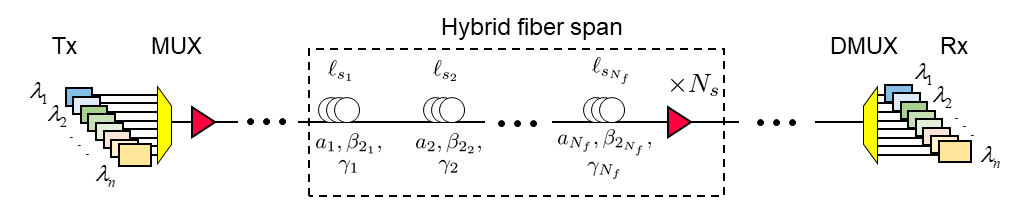
\includegraphics[scale=0.4]{BlockDiagramHybridFiberSpans_Nf.png}
\caption{Hybrid span Model}
\label{fig:hybrid_spans}
\end{figure}


Task 2: Design of multidimensional modulation formats (super-constellations)
We will study multi-dimensional lattice constellations created by taking advantage of more degrees of freedom and therefore more dimensions inherent with MCFs.  We will introduce a new modulation format called mode vector modulation.


Task 3: Modeling and simulation of modal dynamics
We are interested in the study of dynamic random variations of MCFs with weakly-coupled cores. MCF channel dynamics can be simulated by concatenating of random unitary matrices. Rapid channel changes affect the performance of Digital Signal Processing (DSP) algorithms. The ultimate purpose of this task is the performance comparison and the accurate computational complexity evaluation of various DSP algorithms.


\section{Major Activities Done in Academic Year of 2019-2020}

While still and undergraduate student, the MS student took senior-level elective courses that are relevant to the scope of the project: Optical communications, Optoelectronics, and Machine learning. This course work was vital to allow the student to begin working on this project over the summer.

During the summer of 2020 the MS student was familiarized with simulation by using a set of Monte Carlo simulations to simulate the hybrid span model as mentioned earlier. This model had a total length point to point link of 6000 km and does not include modal dynamics. One can see a table of parameters that were tested in Table \ref{tab:param}.  All in all it was over 3000 simulations that needed to be ran to finish the Monte Carlo set. In figure \ref{fig:graphit} to distinguish various simulation cases, we identify individual traces with different colors: fiber configurations with QSMF in the range 0–45 km are shown in pink and the remaining configurations for QSMF in the range 45–100 km per span are shown in cyan. We highlight the extreme cases for 0 km, 45 km, and 100 km using thick red, black, and blue lines respectively.

\begin{figure}
    \centering
    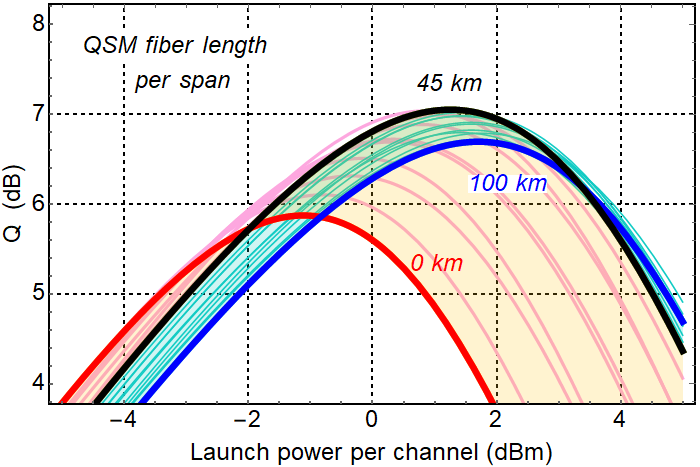
\includegraphics[scale=0.4]{Q0dBvsQSMFlengthplot_6000km_100kmspans_250_112um2_MC_AllTracesPlot_0MPIComp_v02.png}
    \caption{Q-factor as a function of the total launch power per channel for different QSMF lengths per span. (Conditions: System length: 6,000 km, 100 km spans, QSMF effective mode area: 250 $\mu m^2 $, SMF effective mode area: 112 $\mu m^2 $.}
    \label{fig:graphit}
\end{figure}

Once the MS student was trained in the above simulation library he began developing a model capable of simulating modal dynamics. This model was done in MATLAB™ as the student had the most experience in this language and the previous models were also done in MATLAB™ allowing the researchers to add modal dynamics to the previous model and simulation to add more complexity to the previous working model. Modal dynamics are a dynamic random process of cross talk between different modes and channels in MCFs. This was modeled and simulated by concatenating random unitary matrices. This work was done over the summer working directly with the PI. 

The world was changed because of the pandemic of COVID-19. This project was disrupted by the hiring process of foreign students for this research project. Several PhD students who were scheduled to arrive at MSU from abroad in the summer of 2020, before the start of the Fall 2021 semester, were not able to obtain student visas in time. In other cases, travel bans and the worsening pandemic forced some students to cancel or postpone their plans for graduate studies in the US.   
  

% Please add the following required packages to your document preamble:
% \usepackage{booktabs}
% \usepackage{graphicx}
\begin{table}[]
\centering
\caption{Paramters List}
\label{tab:param}
\resizebox{\textwidth}{!}{%
\begin{tabular}{@{}lllll@{}}
\toprule
Span Size(km) & Power Range (dBm) Start & Power Range (dBm) end & MPI Level & Number of Simulations \\ \midrule
10 & -9 & 2 & 0 & 132 \\
20 & -9 & 2 & 0 & 132 \\
25 & -9 & 2 & 0 & 132 \\
30 & -8 & 3 & 0 & 132 \\
40 & -8 & 3 & 0 & 132 \\
50 & -7 & 4 & 0 & 132 \\
60 & -7 & 4 & 0 & 132 \\
75 & -6 & 5 & 0 & 132 \\
80 & -6 & 5 & 0 & 132 \\
120 & -3 & 8 & 0 & 156 \\
150 & -1 & 10 & 0 & 192 \\
10 & -9 & 2 & 100 & 132 \\
20 & -9 & 2 & 100 & 132 \\
25 & -9 & 2 & 100 & 132 \\
30 & -8 & 3 & 100 & 132 \\
40 & -8 & 3 & 100 & 132 \\
50 & -7 & 4 & 100 & 132 \\
60 & -7 & 4 & 100 & 132 \\
75 & -6 & 5 & 100 & 132 \\
80 & -6 & 5 & 100 & 132 \\
120 & -3 & 8 & 100 & 156 \\
150 & -1 & 10 & 100 & 192 \\ \bottomrule
\end{tabular}%
}
\end{table}

\section{Looking Forward}
 During the academic year 2020-2021, to fulfill the MS requirements at MSU, the MS student is taking additional telecommunications courses, i.e., Wireless communications and he is doing an Independent study in advanced topics in Optical Communications. This coursework is closely related to the proposed research topic and, hopefully, will help him succeed in his research goals. It is believed that, after taking these courses, the student will have acquired a solid knowledge of telecommunications and possess useful theoretical skills for doing semi-independent research on the project.

The above course will help the MS student to apply and develop DSP algorithms to current model including; feed-forward equalizers, mode-locked loops, and phase-locked loops. Include Machine learning algorithms such as Artificial Neural networks in lieu of the above DSP algorithms. These algorithms can be included or not included in the simulation of MCFs networks to allow the researchers to better understand how development of multidimensional modulation formats should be done to help recover data loss from the impairments caused by MCFs.

One of the biggest challenges the group faced during the academic year 2019-2020, was restructuring the research activities of the group to a virtual format. The team is currently working in a blended fashion, both on site and remotely. MSU has a state-of-the-art high-performance computing plant. The students have remote access to the servers of this facility. It is anticipated that this facility will remain operational and the students will be able to launch simulations on hundreds of computing nodes remotely.


\section{Stuff from Dr. Roudas}
In one case, a PhD candidate who has been accepted into graduate school had to postpone the beginning of his PhD.


\bibliographystyle{plain}
\bibliography{references}
\end{document}
